%************************************************
\chapter{Theoretical Background}
\label{ch:theory}
%************************************************

\section{Introduction}
Particle physics is a branch of physics that studies the most fundamental particles and their interaction.
We believe that all matter and radiation in the universe are made up of these fundamental particles, and their behaviour is described by the theories in particle physics.
In 20th century, our understanding about the nature of fundamental particles has had great breakthrough and  advance.
Also, many particle colliders have been built to give much insight to develop the theories and test the theories.
The currently mainstream theory of particle physics is called the Standard Model.

\section{Standard Model}
\label{sec:Standard_Model}
Standard Model(SM) is the current theory to describe the fundamental particles in particle physics.
It has already gained huge success in predicting the experimental results, including the prediction of existence of the top quark, the tau neutrino, and the Higgs boson.
It has also explained almost all expermental results with high accuracy.
It represents our best understanding of how the fundamental particles interact with each other.

Physicists discovered that there are 4 fundamental force in the universe: electromagnetic force, weak force, strong force, and gravitational force.
However, SM can only describe 3 of them: electromagnetic, weak and strong interaction, and the gravity cannot be described by SM.
Figure \ref{fig:SM_particles} shows all fundamental particles in SM, and their mass, electric charge and spin.
All matter is made up of fermions (purple and green), which is the first 3 columns in figure \ref{fig:SM_particles}.
Fermions are divided into two groups: quarks(purple) and leptons(green).
The forces between the fermions are mediated by the force carriers, which is gauge bosons(red).
Higgs bosons(yellow) is sclar bosons, which give mass to other massive particles.

\begin{figure}
\centering
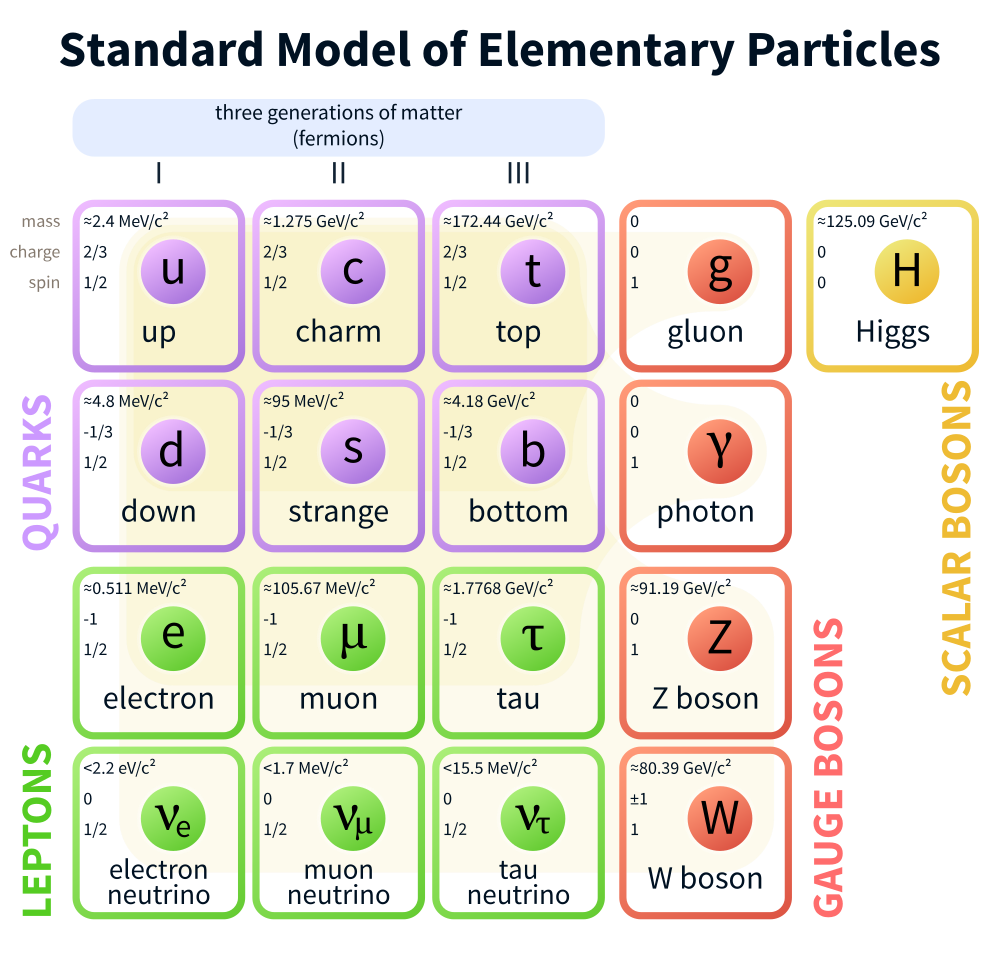
\includegraphics[width=\textwidth]{data/photo/SM_particles.png}
\caption{The table for all fundamental particles in SM. \cite{SM_particles}}
\label{fig:SM_particles}
\end{figure}

\subsection{Matter particles}
There are 6 types of quarks: up quarks(u), down quarks(d), charm quarks(c), strange quarks(s), top quarks(t) and bottom quarks(b).
Quarks interacts with strong interaction, while leptons does not.
There are 3 types of charged leptons: electrons, muons and taus.
There are 3 types of neutral leptons: electron neutrinos, muon neutrinos and tau neutrinos.
The first column is the first generation, which is the lightest and most stable particles.
Hence, normal matter in our daily life is made from the particles in the first generation.
The second and third column are the second and third generation respectively, which is heavier and less stable particles.
These particles will finally decay into the particles in the first generation.
Due to the phenomenon of neutrino oscillation, neutrinos should have non-zero masses, but their value are still uncertain in our current technology.

\subsection{Forces and carrier particles}
Photon is the force carrier for electromagnetic interaction.
Gluon is the force carrier for strong interaction.
Z and W boson is the force carrier for weak interaction.
The effects of these fundamental forces stem from the exchange of the corresponding force carrier.
These forces also have different strengths and different ranges.
Strong force is the strongest force, while the electromagnetic force is in the middle.
The weak force is the weakest force among the three, but it still much much stronger that the gravity.
The electromagnetic force has infinite range, while the strong and weak forces have very short ranges at the level of subatomic particles.

For example, a proton is composed of two up quarks and one down quark, and a neutron is composed of onw up quark and two down quarks.
The forces between quarks inside the proton are mediated by gluons.

\subsection{Feynman diagram}
The fundamental interactions among these fundamental particles are described by the allowed fundamental Feynman vertices.
All allowed fundamental Feynman vertices in SM are shown in figure \ref{fig:vertices_SM} and \ref{fig:vertices_higgs}.
These fundamental vertices are the basic building blocks for all physical processes, by jointing these vertices together.

\begin{figure}
\centering
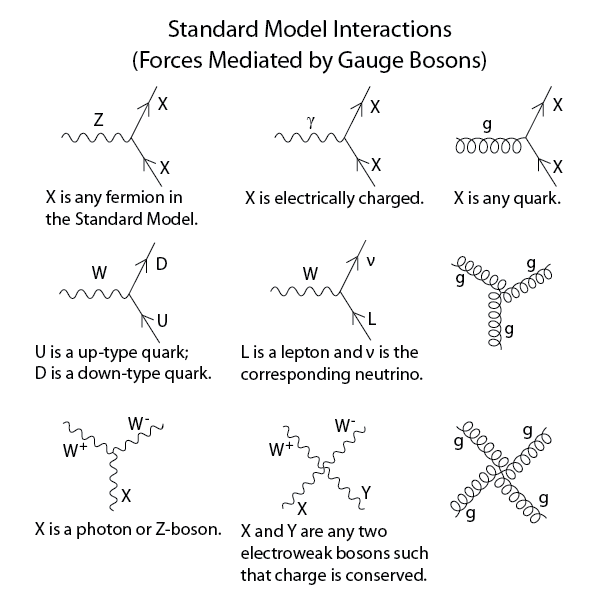
\includegraphics[width=\textwidth]{data/photo/vertices_SM.png}
\caption{All allowed fundamental Feynman vertices in SM, except higgs-related vertices. \cite{vertices_SM}}
\label{fig:vertices_SM}
\end{figure}

\begin{figure}
\centering
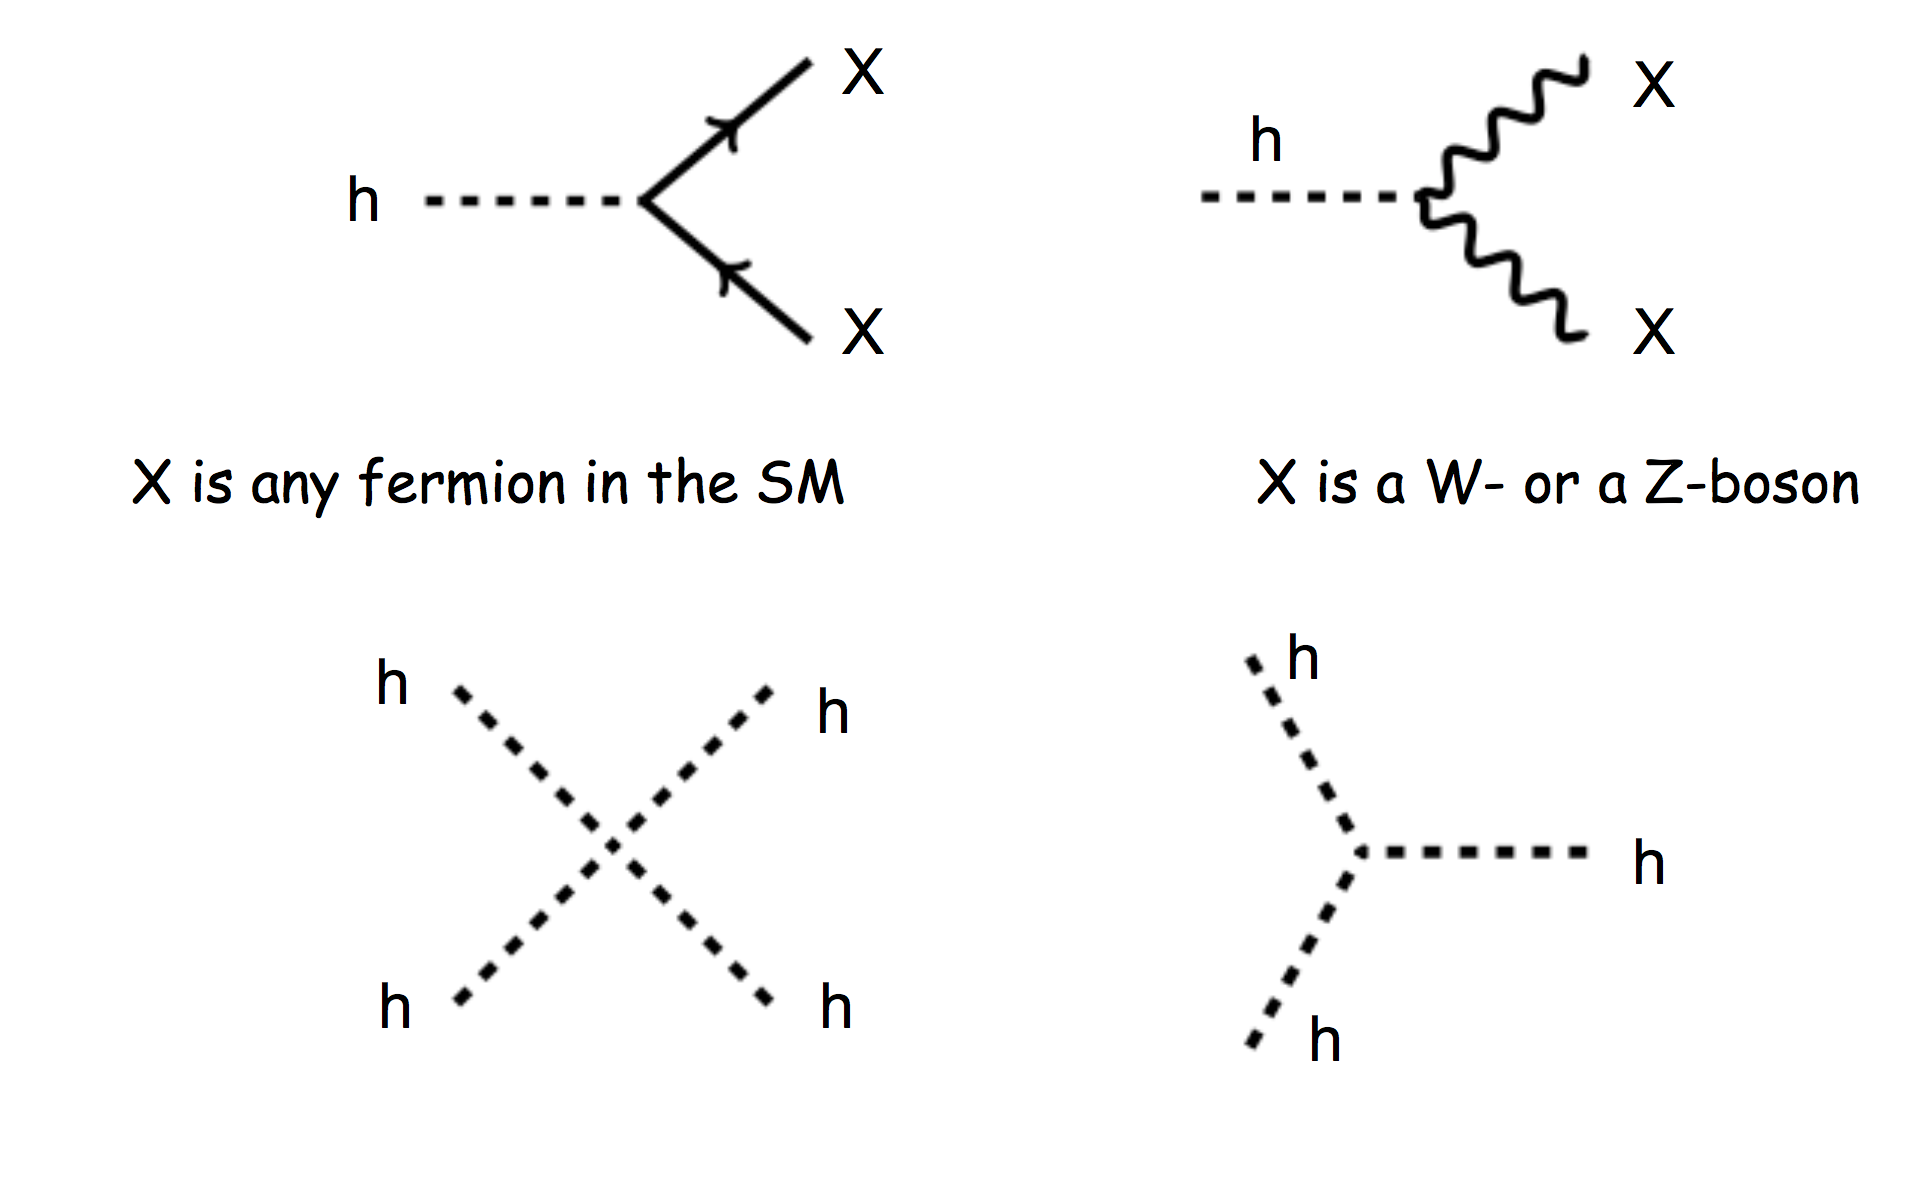
\includegraphics[width=\textwidth]{data/photo/vertices_higgs.png}
\caption{All allowed fundamental higgs-related Feynman vertices in SM.}
\label{fig:vertices_higgs}
\end{figure}

\section{Limitation of Standard Model}
\label{sec:Limitation_Standard_Model}
Although Standard Model can explain almost all experimental results, there still are some phenomena it cannot explain.

\subsection{Dark matter}
Dark matter is some unknown matter that does not involve in electromagnetic interaction, but involve in gravitational interaction.
It was first discovered in the Milky Way, by studying the speed of the stars orbiting around the center of the Milky Way.
Because it does not involve in electromagnetic interaction, it does not emit any electromagnetic radiation, and it cannot be seen by our telescopes.
However, SM cannot explain the nature of dark matter, and what dark matter is made of.

\subsection{Hierarchy problem}
\label{subsec:hierarchy_problem}
The hierarchy problem is the question why the weak force is stronger than the gravitational force by $10^{24}$ times.
It is also asked why the mass of Higgs boson ($\sim 125$ GeV) is much lighter than the Planck mass ($\sim 10^{19}$ GeV).

The Lagrangian for the interaction term between the fermion Dirac field $\psi$ and the Higgs field $h$ (i.e. Yukawa interaction) is given by
\begin{equation}
\mathcal{L}_{\text{Yukawa}} = - \lambda \bar{\psi} h \psi
\end{equation}
where $\lambda$ is the Yukawa coupling constant.
The quantum correction to the square of the Higgs mass $\Delta m^2_H$ is then given by
\begin{equation}
\Delta m^2_H = - \frac{|\lambda|^2}{16 \pi^2} \Lambda^2 + \dots
\label{eq:higgs_correction}
\end{equation}
where $\Lambda$ is the energy scale up to which the Standard Model is valid, namely the Planck scale ($\sim 10^{19}$ GeV).
Because $\Lambda$ is quadratic divergent, the correction to the Higg mass is in the order of Planck scale.
Unless there are very delicate cancellation between the correction terms, the Higgs mass should be in the order of Planck scale.
But, we found that the experimental Higgs mass is in the order of 125 GeV, and this is called the hierarchy problem.

\subsection{Unification of forces}
In the 1860s, James Clerk Maxwell wrote down his famous equations Maxwell's equations, which unified two different phenomena: electricity and magnetism.
Due to this unification, we now understand that electricity and magnetism are two different manifestations of the same phenomenon, and we now call it electromagnetism.

Similar thing happened in 1970s, physicists developed a theory that unified two fundamental forces: electromagnetic force and weak force.
At the energy scale above 246 GeV, these two forces will merge into a single force: electroweak force.
This unification predicted the existence of weak neutral current and a force carrier to carry this weak force.
This force carrier was later comfirmed experimentally in CERN, and it is now called the Z boson.

After that, an effect of strong force was found experimentally that the strong force becomes weaker when the energy is higher.
This may indicate that electroweak force and strong force will become a single force at even high energy.
However, the energy scale at which these forces are the same is much larger than the energy the particle accelerators can reach.
There are some theories beyond the Standard Model that try to unify these force, such as supersymmetry.

\section{Supersymmetry}
Supersymmetry(SUSY) is an extension of the Standard Model, and try to answer some questions which the Standard Model cannot explain mentioned in section \ref{sec:Limitation_Standard_Model}.
One of the problem SUSY can solve is the hierarchy problem of Higgs mass mentioned in section \ref{subsec:hierarchy_problem}.
We first notice that the negative sign in the equation \ref{eq:higgs_correction} is due to the correction from the fermions.
If we can somehow have some symmetry between the fermions and bosons, and add more positive correction terms due to the bosons, the correction terms will cancel with each other and the hierarchy problem can be solved.
This new symmetry is called the supersymmetry(SUSY).

\subsection{Minimal Supersymmetric Standard Model}
Minimal Supersymmetric Standard Model(MSSM) is the minimal supersymmetrical theory that contain the least number of new particle states and new interactions.
It predicts that each particle in the Standard Model has its own partner particle, called the superpartner.
The name of the superpartner is by adding a prefix "s", followed by the name of the orginal Standard Model particle.
For example, the superpartner of an electron is called selectron.
As for the symbol for the superpartner, a tilde will be added above the original symbol.
For example, the symbol for selectron is $\tilde{e}$.
Also, the spin of the superpartner will differ from the Standard Model particle by 1/2.
For fermions, the spin of their superpartner is 0, while for bosons, the spin of their superpartner is 1/2.
This is the new symmetry between the fermions and bosons, mentioned before.
It is also the correction terms from these superpartners to fix the hierarchy problem of the Higgs mass.
If MSSM is correct, these supersymmetric particles should be detected in the LHC.

\section{Wh channel}
\begin{figure}
\centering
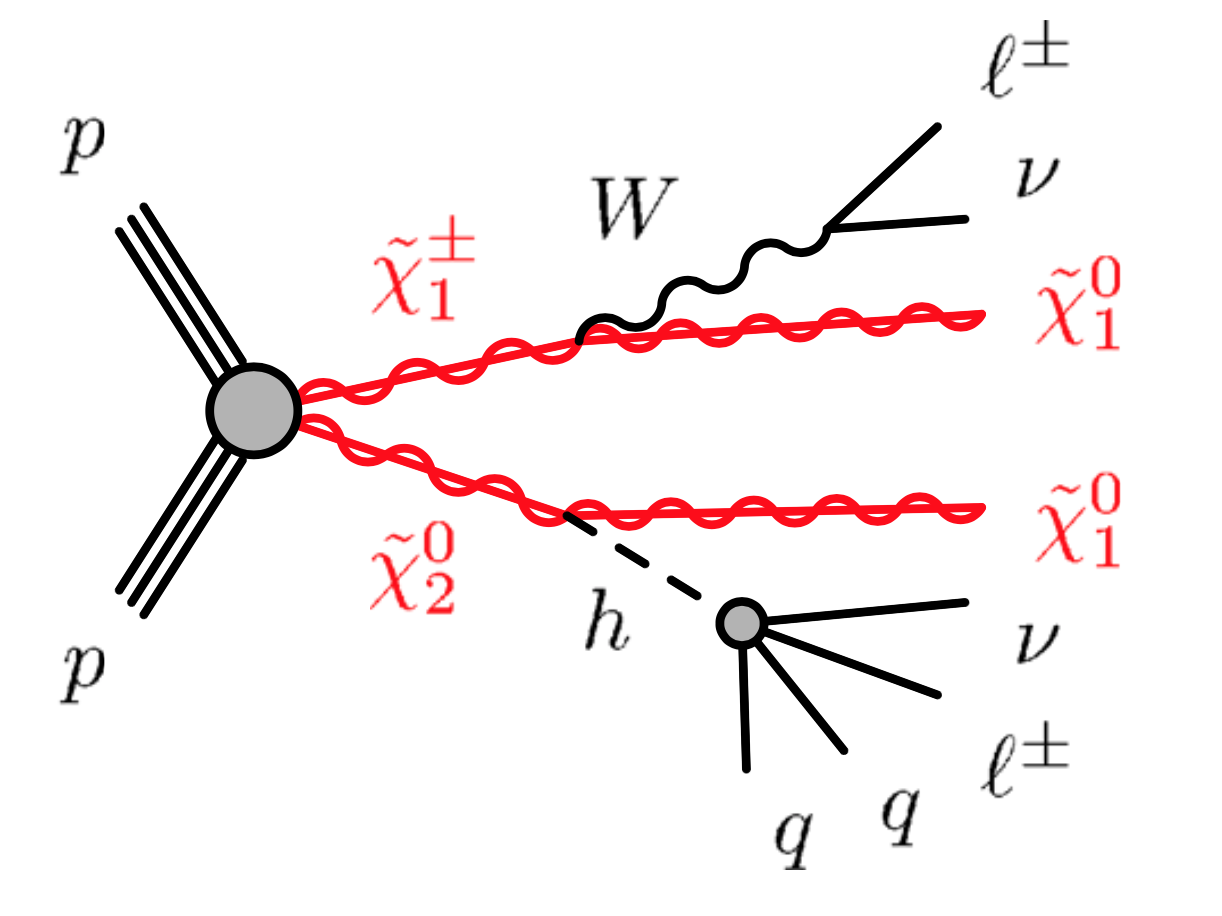
\includegraphics[width=0.5\textwidth]{data/photo/theory/signal_feynman.png}
\caption{The Feynman diagram for our Wh signal}
\label{fig:signal_feynman}
\end{figure}


